\documentclass[13pt, usenames, dvipsnames]{beamer}
\usepackage{pgfpages}

%\setbeameroption{show notes on second screen}
\usetheme[progressbar=frametitle,block=fill]{metropolis}

%\usepackage[
%backend=biber,
%style=ieee,
%citestyle=authoryear,
%mincitenames=1,
%maxcitenames=1
%]{biblatex}

\usepackage{alltt}
\usepackage{tikz, verbatimbox}
\usetikzlibrary{arrows, arrows.meta, positioning, decorations.markings, shapes, decorations, overlay-beamer-styles}
\usepackage{xcolor}
\usepackage[utf8]{inputenc}
\usepackage{multicol}
\usepackage{tabularx}
\usepackage{marvosym} 
\usepackage{comment}
\usepackage[ngerman]{babel}

%\addbibresource{bib.bib}

\tikzset{>=Latex}
\tikzset{
  %auto,
  invisible/.style={opacity=0},
  visible on/.style={alt={#1{}{invisible}}},
  alt/.code args={<#1>#2#3}{%
    \alt<#1>{\pgfkeysalso{#2}}{\pgfkeysalso{#3}} % \pgfkeysalso doesn't change the path
  },
}

\newcommand\Wider[2][2.0cm]{%
\makebox[\linewidth][c]{%
  \begin{minipage}{\dimexpr\textwidth+#1\relax}
  \raggedright#2
  \end{minipage}%
  }%
}

\begin{document}
\begin{frame}{Offene Daten für personalisierte Stadexploration}
    \begin{minipage}{.5\textwidth}
        \only<1>{\includegraphics[width=\textwidth]{großerGarten.png}}
        \only<2>{\includegraphics[width=\textwidth]{frauenkircheAusblick.png}}
        \only<3>{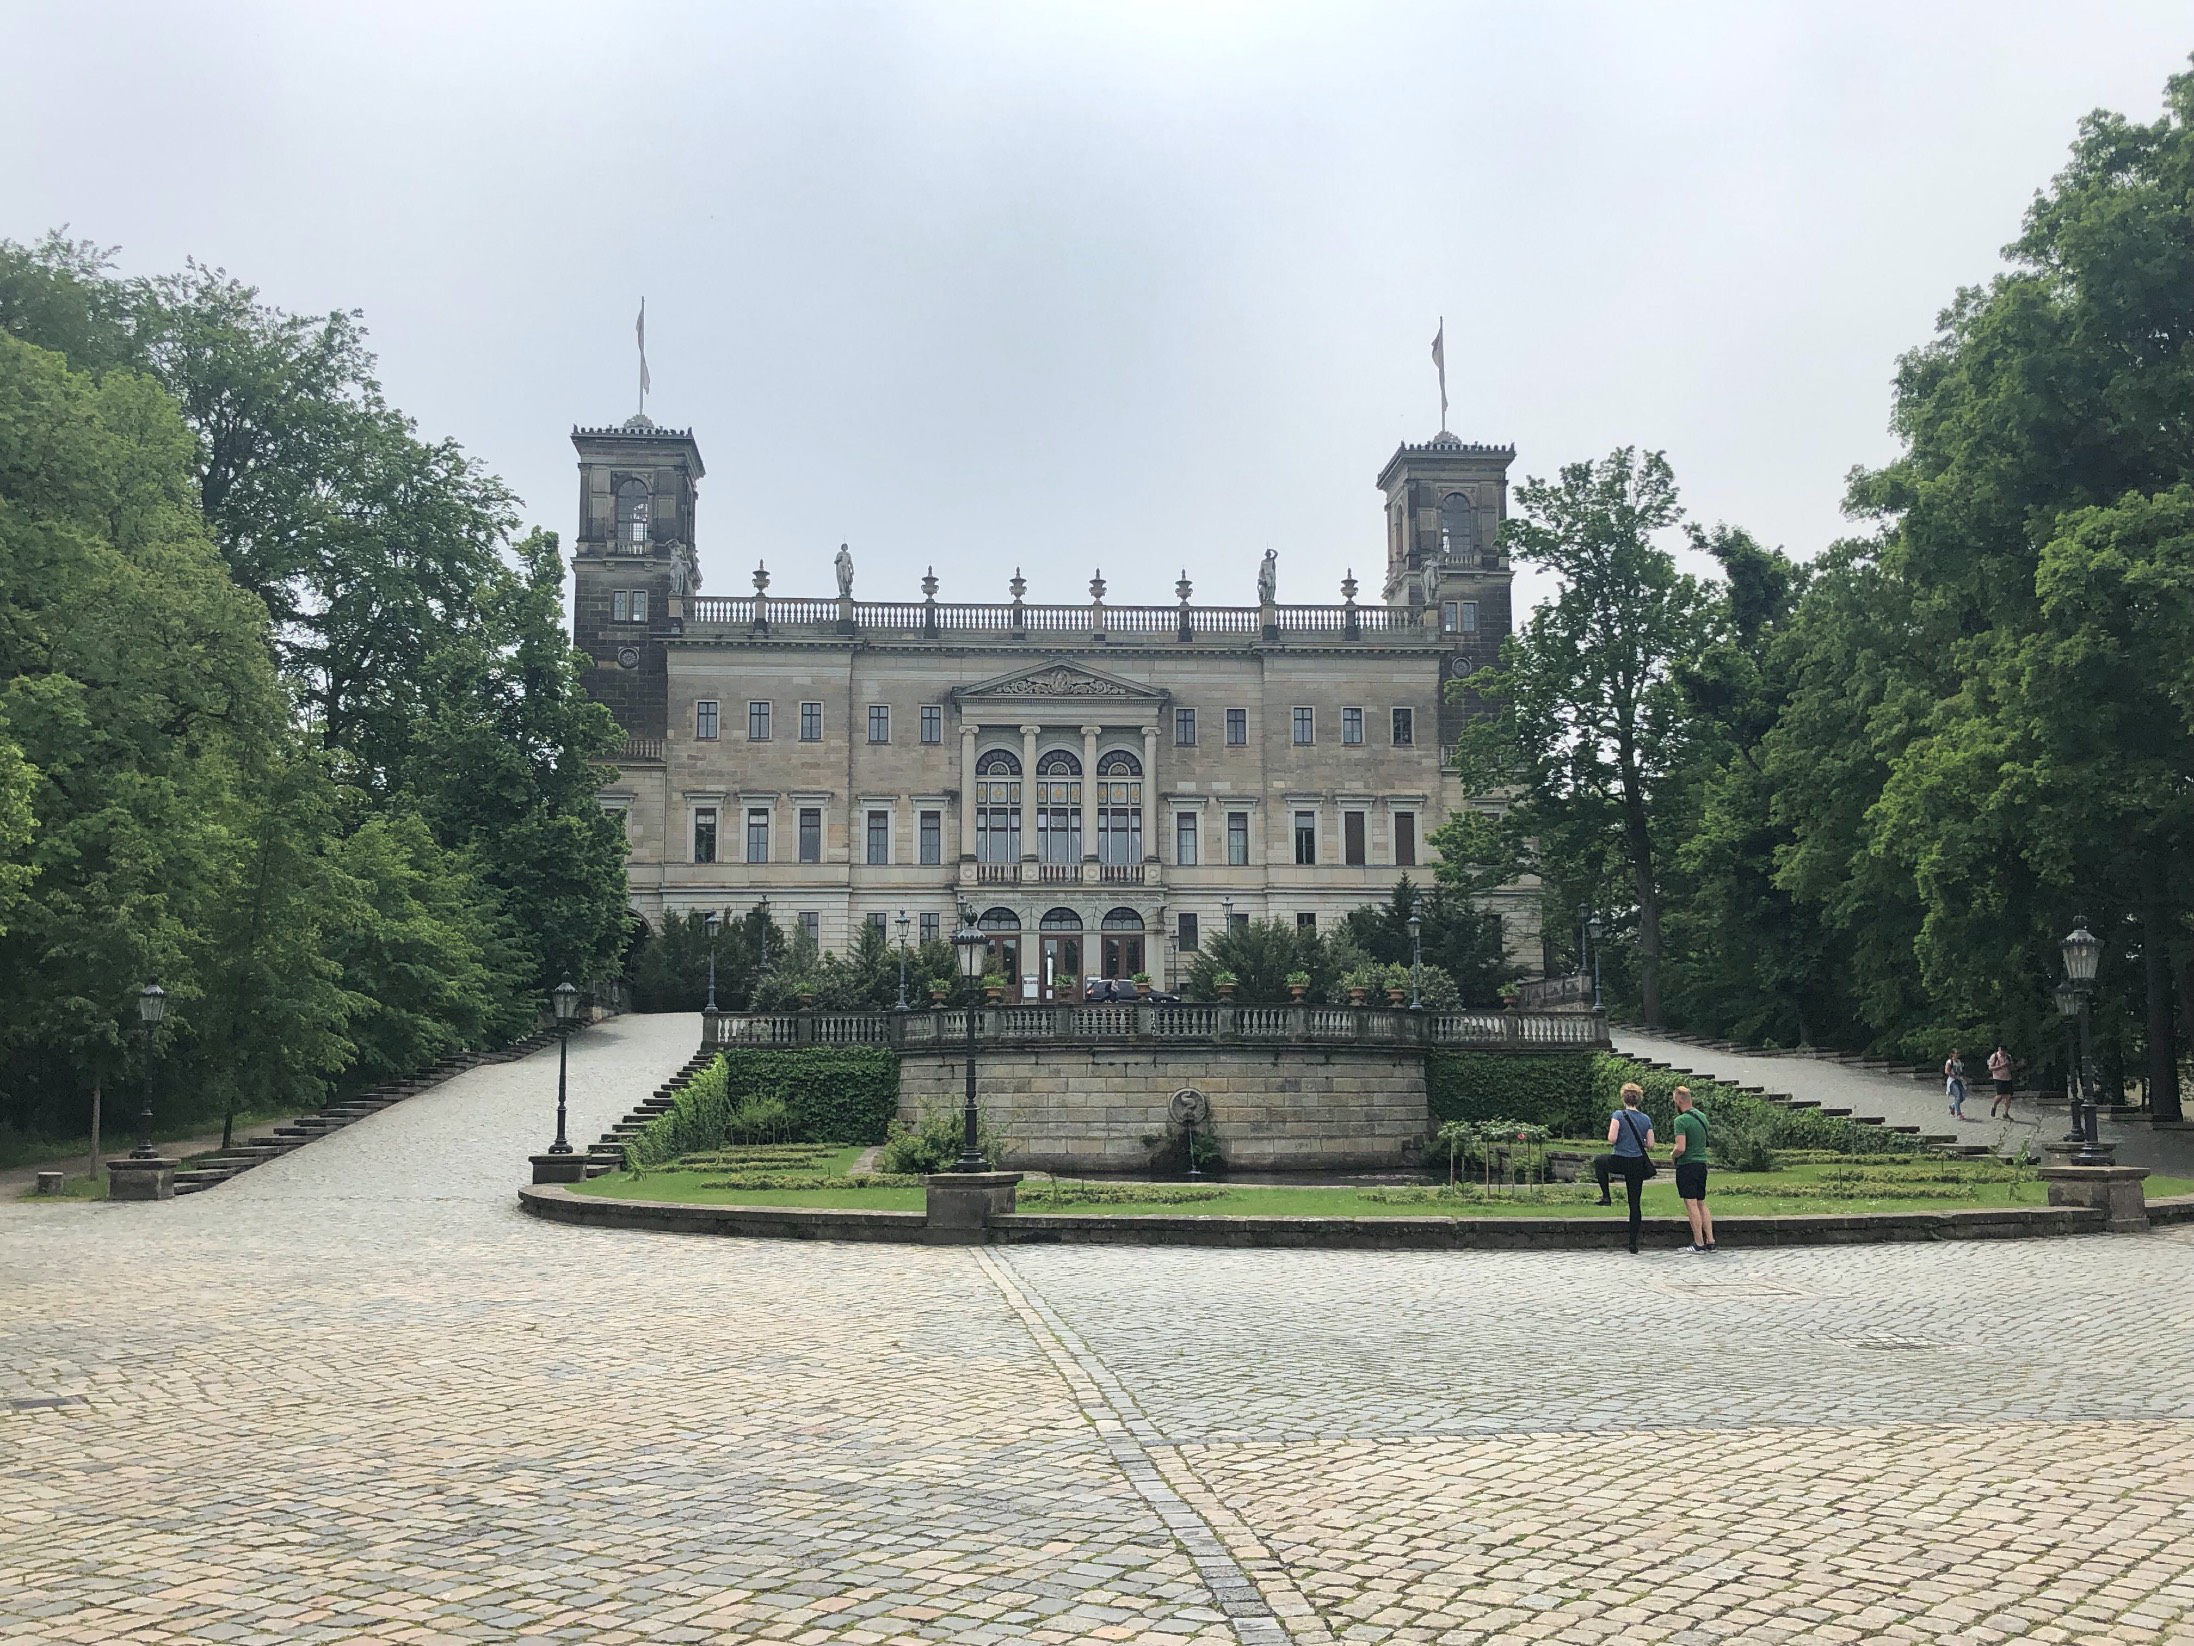
\includegraphics[width=\textwidth]{albrechtsbergSchloss.png}}
    \end{minipage}%
    \begin{minipage}{.5\textwidth}
        \begin{itemize}
            \item Die eigene Stadt neu entdecken
                \pause
            \item Personalisierte Ziele für Touristen
                \pause
            \item Anbieten von Bildungstouren
        \end{itemize}
    \end{minipage}
\end{frame}

\begin{frame}{Rundrouten}
    Rundrouten erklären
\end{frame}

\begin{frame}{Wen wollen wir erreichen?}
    \begin{itemize}
        \item Einheimische, die Dresden neu entdecken wollen.
        \item Touristen, die für sie interessante Ziele besuchen wollen.
        \item Die Stadt als Anbieter / Planer für kulturelle Stadttouren.
    \end{itemize}
\end{frame}

\begin{frame}{}
    \begin{tikzpicture}
        \node[draw] (data) at (-3, 0) {Datenauswahl};
        \node[draw] (routing) at (0, 0) {Routing};
        \node[draw] (vis) at (3, 0) {Visualisierung};

        \draw[->] (data) -- (routing);
        \draw[->] (routing) -- (vis);
    \end{tikzpicture}
\end{frame}
\end{document}
